\section{Défis techniques du Hardware}
Le hardware doit pouvoir manipuler des plaques de microcapsules ou de réacteurs, ainsi que des microcapsules en verre de $\qty{3}{\mm}$ de diamètre en garantissant leur intégrité. Le tout doit être dans un espace confiné.
\section{Recherches de solution}
Pour la recherche des solutions, le hardware a été décomposé par les fonctions suivantes : 
\begin{itemize}
    \item Saisie et dépose des microcapsules;
    \item déplacement des microcapsules;
    \item saisie et dépose des plaques.
\end{itemize} 
La position des plaques dans la glove box a également été étudié avec $6$ configurations différentes.
\subsection{Saisie et dépose des microcapsules}
Pour la saisie des microcapsules, les grandes familles de solutions proposées sont : 
\begin{itemize}
    \item Aspiration;
    \item Mécanique; \begin{itemize}
        \item Pince à doigt;
        \item Pince Gecko.
    \end{itemize}
\end{itemize}
\subsubsection*{Avantage et inconvénients}
\begin{table}[H]
    \caption{Avantages et inconvénients des solutions de saisie des microcapsules}
    \begin{tabular}{@{}cll@{}}
    \toprule
    Solution      & \multicolumn{1}{c}{Avantages}                                                                                                   & \multicolumn{1}{c}{Inconvénient}                                                                                                                                  \\ \midrule
    Aspiration    & \begin{tabular}[c]{@{}l@{}}- Exerce moins de pression directe \\ - Simple à installer\\ - Nécessite peu d'entretien\end{tabular} & \begin{tabular}[c]{@{}l@{}}- Apporter l'énergie pneumatique\\ - Bruyant\end{tabular}                                                                     \\
    Pince à doigt & \begin{tabular}[c]{@{}l@{}}- Contrôle précis\\ - Faible coût\end{tabular}                                                        & \begin{tabular}[c]{@{}l@{}}- Maintenance fréquente\\ - Ne convient pas au petits objets\\ - Espace limité, pour pouvoir ouvrir \\ et fermer la pince \\ - Nécessite un contrôle de force\end{tabular} \\
    Pince Gecko   & \begin{tabular}[c]{@{}l@{}}- Saisie non intrusive\\ - Ne nécessite pas de source \\ d'énergie externe\end{tabular}                            & \begin{tabular}[c]{@{}l@{}}- Capacité de charge\\ - Nécessite un nettoyage pour maintenir \\  l'adhérence\\ - Détachement complexe\end{tabular}     \\ \bottomrule
    \end{tabular}
\end{table}
\subsection{Déplacement des microcapsules}
Pour le déplacement des \glspl{microcapsule} de leur plaque jusqu'aux réacteurs, trois idées ont été étudiées : 
\begin{itemize}
    \item Transport pneumatique par tube;
    \item convoyeur;
    \item robot.
\end{itemize}
\subsection*{Transport pneumatique par tube}
Le système de transport pneumatique par tube, serait des tuyaux dans lesquelles naviguent les \glspl{microcapsule} grâce à une différence de pression de chaque côté de la \gls{microcapsule}. Ce système est déjà présent dans les hôpitaux et dans les grandes surfaces.
\begin{figure}[h!]
    \centering
    \begin{subfigure}{0.45\textwidth}
        \centering
        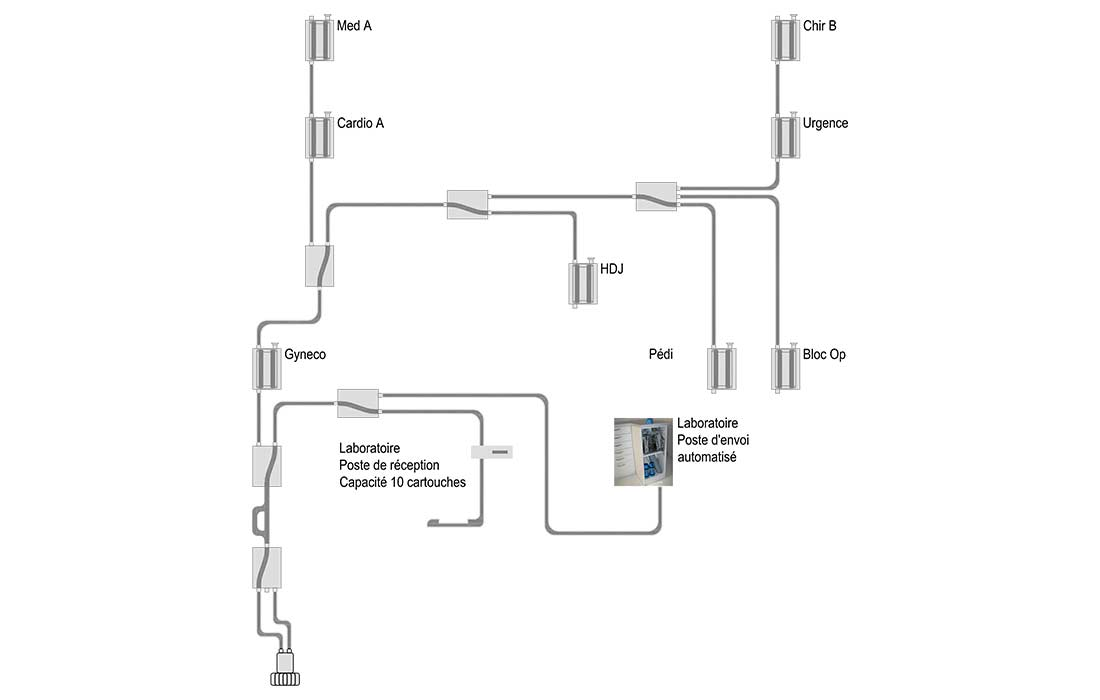
\includegraphics[width=\linewidth]{assets/figures/Hardware/transport_pneu/reseau_pneumatique_hopital.jpg}
        \caption{Schéma d'un réseau de transport pneumatique\footnotemark}
    \end{subfigure}\hfill
    \begin{subfigure}{0.45\textwidth}
        \centering
        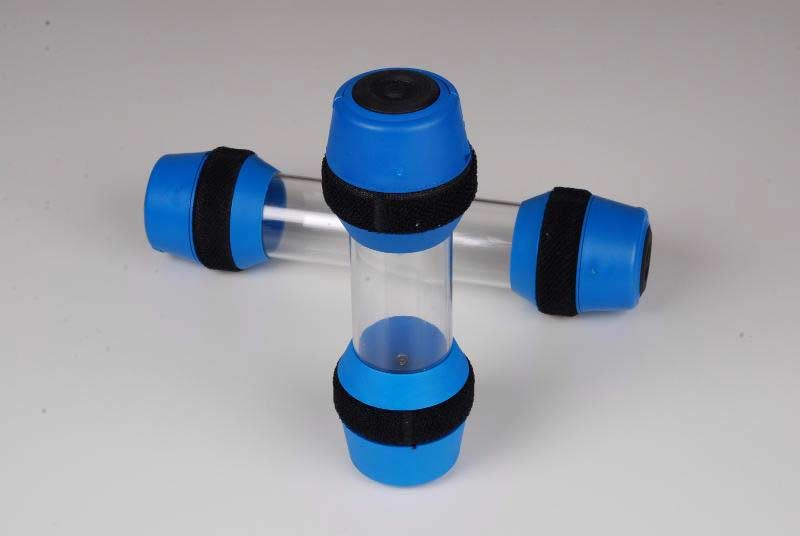
\includegraphics[width=\linewidth]{assets/figures/Hardware/transport_pneu/cartouche_transport_pneu.jpg}
        \caption{Cartouche de transport\footnotemark}
    \end{subfigure}
    \caption{Exemples de réseau de transport pneumatique par tube}
\end{figure}
\footnotetext[1]{\href{https://www.transport-pneumatique.fr/transport-pneumatique-centres-hospitaliers/}{https://www.transport-pneumatique.fr/transport-pneumatique-centres-hospitaliers/}}
\footnotetext[2]{\href{https://www.transport-pneumatique.fr/cartouches-pochettes/}{https://www.transport-pneumatique.fr/cartouches-pochettes/}}
\subsection*{Transport par convoyeur}
Pour déplacer les \glspl{microcapsule}, un convoyeur peut être utilisé, il faut néanmoins que le convoyeur soit adapté au \gls{microcapsule}, les \glspl{microcapsule} étant cyclindriques, elles risquerait de rouler sur un convoyeur à bande lisse, mais une bande à tasseau (\cf \autoref{img:convoyeur_bande_tasseau}) ou un demi-tube  (\cf \autoref{img:convoyeur_tube}) conviendraient parfaitement.
\begin{figure}[h!]
    \centering
    \begin{subfigure}{0.45\textwidth}
        \centering
        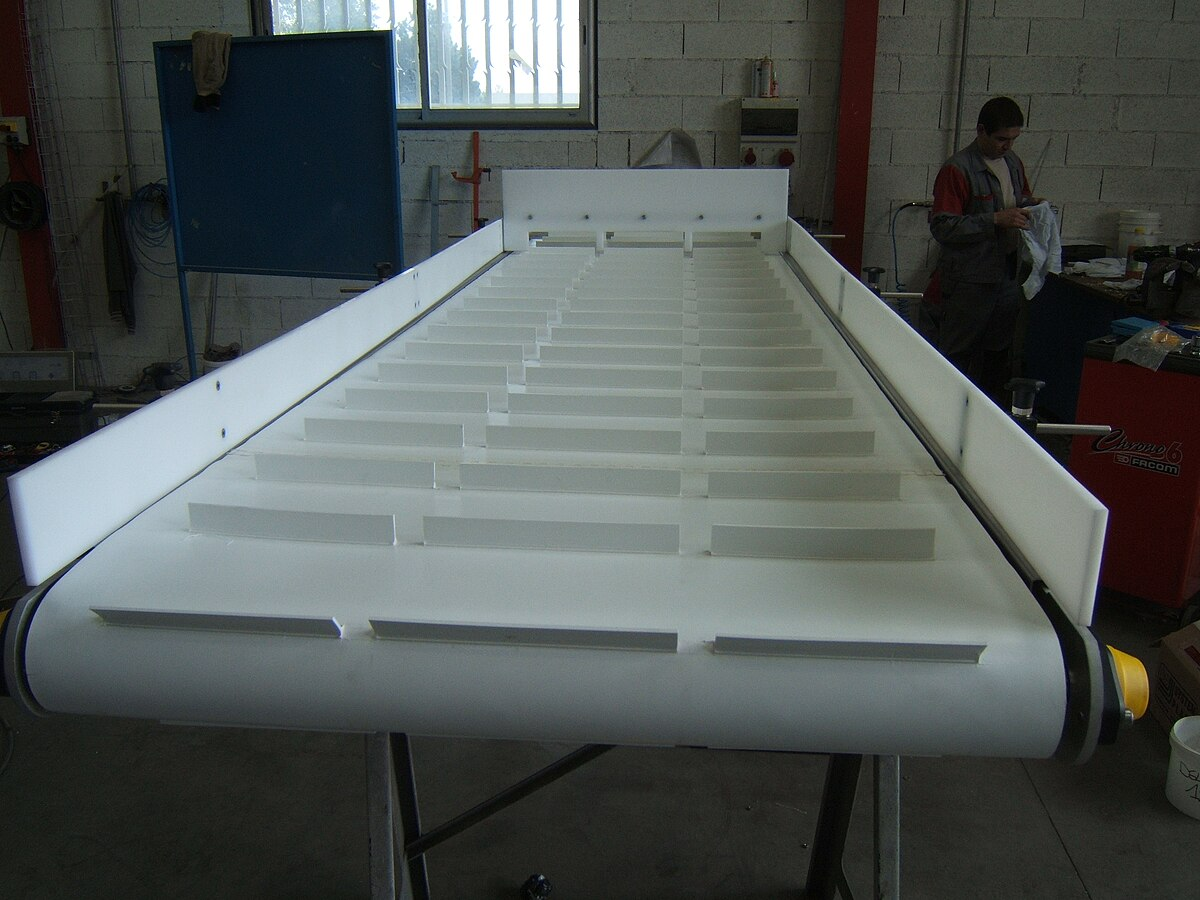
\includegraphics[width=\linewidth]{assets/figures/Hardware/transport_conv/convoyeur_tasseau.JPG}
        \caption{Convoyeur avec bande à tasseaux\footnotemark}
        \label{img:convoyeur_bande_tasseau}
    \end{subfigure}\hfill
    \begin{subfigure}{0.45\textwidth}
        \centering
        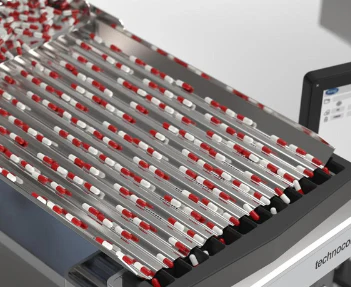
\includegraphics[width=\linewidth]{assets/figures/Hardware/transport_conv/convoyeur_tube.png}
        \caption{Convoyeur à tube\footnotemark}
        \label{img:convoyeur_tube}
    \end{subfigure}
    \caption{Exemple de convoyeur}
\end{figure}
\footnotetext[2]{\href{https://fr.m.wikipedia.org/wiki/Convoyeur}{https://fr.m.wikipedia.org/wiki/Convoyeur}}
\footnotetext[3]{\href{https://doser-compter.com/products/ligne-de-comptage-king}{https://doser-compter.com/products/ligne-de-comptage-king}}
Quant aux différents moyens de mouvoir les \glspl{microcapsule}, il y a : 
\begin{itemize}
    \item les vibrations;
    \item le déplacement de la bande;
    \item la gravité.
\end{itemize}

La dernière option nécessite des surface lisses, que le système soit en pente et le temps de déplacement n'est pas réglable. Les deux autres solutions ne se distinguent pas vraiment pour l'instant, car dans tous les cas, l'utilisation d'un moteur électrique est nécessaire.

\subsection*{Déplacement à l'aide d'un robot}
Pour le déplacement des \glspl{microcapsule}, seuls les axes $T_x, T_y~\text{et}~T_z$ sont nécessaires, soit $3$ degrés de liberté. Un robot de type \textit{SCARA}, cylindrique ou Delta peuvent correspondre.

\subsection*{Avantages et inconvénients}
\begin{table}[H]
    \caption{Anvantages et inconvénients des solution de transport des \glspl{microcapsule}}
    \begin{tabular}{@{}cll@{}}
    \toprule
    Solution      & \multicolumn{1}{c}{Avatanges}                                                                                                   & \multicolumn{1}{c}{Inconvénient}                                                                                                                                  \\ \midrule
    Transport pneumatique par tube    & \begin{tabular}[c]{@{}l@{}}\end{tabular} & \begin{tabular}[c]{@{}l@{}}- Peu modulable\\ - Bruyant\\ - Aiguillage complexe\end{tabular}                                                                     \\
    Convoyeur & \begin{tabular}[c]{@{}l@{}}- \\ - \end{tabular} & \begin{tabular}[c]{@{}l@{}}- Maintenance fréquente\\ - Ne convient pas au petits objets\\ - Espace limité, pour pouvoir ouvrir \\ et fermer la pince \\ - Nécessite un contrôle de force\end{tabular} \\
    Robot   & \begin{tabular}[c]{@{}l@{}}- Place\\ - Modulable \\ \end{tabular}                            & \begin{tabular}[c]{@{}l@{}}- Coût\\ - Nécessite un nettoyage pour conserver \\  l'adhérence dans le temps\\ - Détachement complexe\end{tabular}     \\ \bottomrule
    \end{tabular}
\end{table}

\subsection{Analyse des solutions}
De par la complexité et le manque de modularité du transport pneumatique et du convoyeur, le choix d'utiliser un robot a été choisi.

La position des plaques dans la \textit{glove box} est importante pour la suite, elle permettra de choisir le type de robot à utilisés.
Il est important de savoir comment placer les deux plaques dans la \textit{glove box}.
\subsubsection{Positionnement des plaques dans la \textit{glove box}}
Pour la position des plaques, les solutions trouvées sont : 
\begin{enumerate}
    \item Les plaques ne bougent pas et restent dans les sas;
    \item Les plaques sont positionées symétriquement par rapport au centre de la \textit{glove box};
    \item La plaque de microcapsules est déplacée à côté de la plaque de réacteur, cette dernière ne bouge pas;
    \item La plaque de microcapsules reste dans le sas tandis que la plaque de réacteur est transportée à ses côtés;
    \item Les deux plaques sont mises l'une à côté de l'autre en étant plus proches du stock;
    \item Les deux plaques sont mises l'une à côté de l'autre en étant plus proches de la sortie;
\end{enumerate}
Le temps de cycle est le suivant :
\begin{align*}
    tpsCycle &= tpsDeplacementPlaquesCapsule + tpsDeplacement_{Capsule} \\
    &+ tpsAttentePlaque + tpsDeplacement_{PlaquesReacteur}\\
    &= nbrePlaques\cdot \frac{d_{PlaqueMicrocapsules}}{v_{robot}} + nbreMicrocapsules\cdot \frac{d_{EntrePlaque}}{v_{robot}} \\
    &+ 2\cdot nbrePlaques\cdot tpsAttente + \frac{d_{PlaqueReacteur}}{v_{robot}}
\end{align*}

Certaines valeurs ne peuvent être connue que lors de la mise en route, notamment l'accélération, la vitesse d'approche, il est nécessaire de faire certaines hypothèses. Les distances sont également arbitraires afin de se faire une idée du temps de cycle des solutions. Ici, la position optimale n'est pas recherché.
En utilisant les hypothèses suivantes :
\begin{itemize}
    \item $v_{robot} = \qty{1}{\frac{\m}{\s}}$;
    \item $d_{EntrePlaque} = \qtylist[list-units = single]{1.33; 0.3; 0.3; 0.3; 0.3; 0.3}{\m\per\s}$;
    \item $d_{PlaqueMicrocapsules} = \qtylist[list-units = single]{0; 0.515; 1.03; 0; 0.83; 0.2 }{\m}$;
    \item $d_{PlaqueReacteur} =      \qtylist[list-units = single]{0; 0.515; 0; 1.03; 0.2; 0.83 }{\m}$;
    \item $d_{PlaqueMicrocapsules} = \qtylist[list-units = single]{0; 0.515; 1.03; 0; 0.83; 0.2 }{\m}$;
    \item L'accélération du robot est infinie;
    \item La vitesse d'approche n'est pas prise en compte.
\end{itemize}
Avec ces informations, il est possible de calculer le temps moyen d'un cycle (\cf \autoref{img:graph_temps_cycle_moyen_sequentielle}) en fonction du nombre de microcapsule demandées ainsi que du nombre de microcapsule par plaque, et ce, pour chaque solution.
\begin{figure}[H]
    \centering
    \includesvg[width = \textwidth]{assets/figures/Hardware/recherchSoluce/temps_cycle_moyen_toute_solution.svg}
    \caption{Temps de cycle moyen des différentes solutions}
    \label{img:graph_temps_cycle_moyen_sequentielle}
\end{figure}
Il est possible de voir que les solutions $1$ et $6$ semble les plus rapide. Le temps d'attente des plaques est cependant très important, environ $84~\%$ du temps total. Pour réduire ce délai, il peut être intéressant de paralléliser les tâches.
\subsubsection{parallélisation des robots}
La parallélisation des tâches consiste à effectuer le \textit{pick and place} des microcapsules, la prise et la dépose des plaques indépendamment.
De par la configuration des sas, il n'est possible d'y mettre qu'une seule plaque, la parallélisation des solutions $\numlist{1; 3; 4}$ n'est donc pas possible.

\begin{figure}[H]
    \centering
    \includesvg[width = \textwidth]{assets/figures/Hardware/recherchSoluce/para.svg}
    \caption{Comparaison du temps de cycle des solutions en fonction du nombre de microcapsules par plaque}
    \label{img:graph_temps_cycle_para}
\end{figure}

Sur \autoref{img:graph_temps_cycle_para}, il est possible de voir que les solutions parallélisées ont toujours un temps de cycle inférieur aux solutions séquentielles tant que le nombre de microcapsules par plaque est inférieur au nombre de microcapsules demandées.
Plus le nombre de microcapsule demandées est élevé, plus le gain de temps est significatif, allant, en moyenne, de $1.3~\%$ pour $48$ microcapsules à $27~\%$ pour $240$ microcapsules.
\section{Présentation de la solution choisie}
L'utilisation d'un seul robot positionné au centre de la \textit{glove box}, qui s'occupera de déplacer les plaques ainsi que de faire le \textit{pick and place} des microcapsules a été retenue.
Cette décision est due à : 
\begin{itemize}
    \item un robot déjà présent dans le laboratoire;
    \item la grande flexibilité de cette solution (la \textit{glove box} sera utilisée pour d'autres processus par la suite).
\end{itemize}
\section{Description du matériel utilisé}
Voici la liste de matériel utilisé lors du TB : 
\begin{itemize}
    \item Robot \og{}UR3e\fg{};
    \item Pince \og{}Hand-E\fg{};
    \item Adaptation de la pince précédente sur mesure;
    \item Module d'aspiration;
    \item Support pour les plaques.
\end{itemize}
\section{Intégration}
Afin de maximiser l'espace accessible par le robot, il a été surélevé (\cf \autoref{img:integration_robot_glove}). La moitié gauche est réservée pour le \textit{pick and place} des microcapsules, tandis que la partie à droite servira pour la suite du processus.
Pour les outils, la pince se met sur la bride du robot et elle possède deux trous taraudés qui seront utilisé pour fixer le module d'aspiration (\cf \autoref{img:integration_pince}).
L'outil pour saisir les plaques fait un angle à $\qty{45}{\degree}$ pour pouvoir déposer les plaques sur tout le plan \textit{repPickAndPlace}. Afin de gagner de la place, les deux outils sont placés dans des directions opposées.
\begin{figure}[]
    \centering
    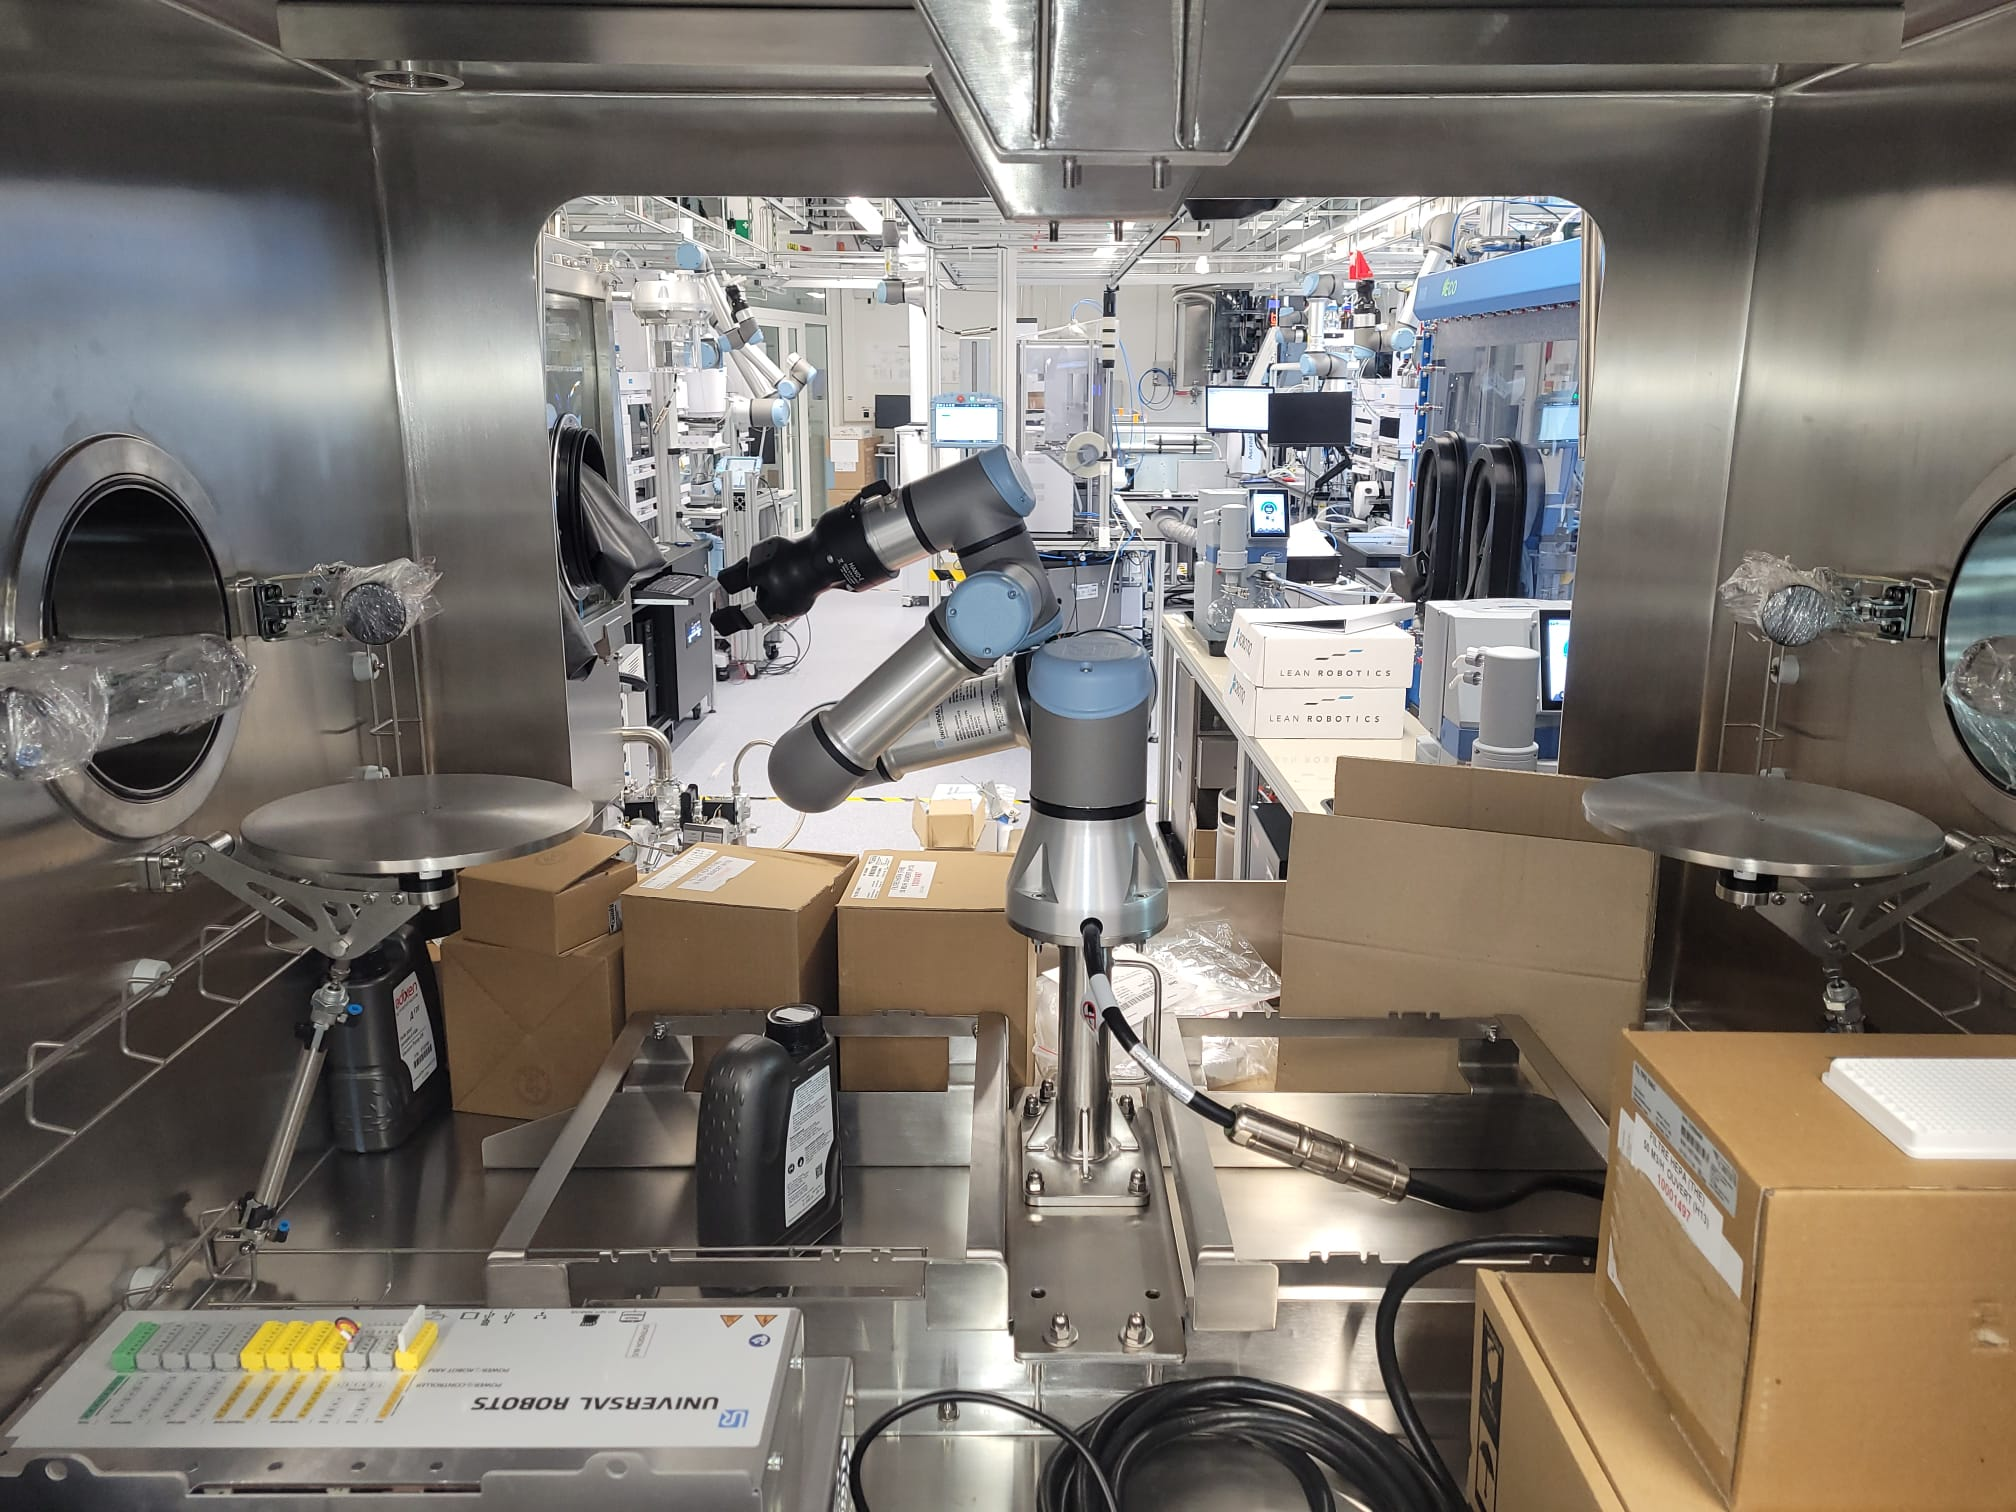
\includegraphics[width = 0.5\textwidth]{assets/figures/Hardware/gloveBox.jpeg}
    \caption{Intégration du robot dans la \textit{glove box}}
    \label{img:integration_robot_glove}
\end{figure}
\begin{figure}[]
    \centering
    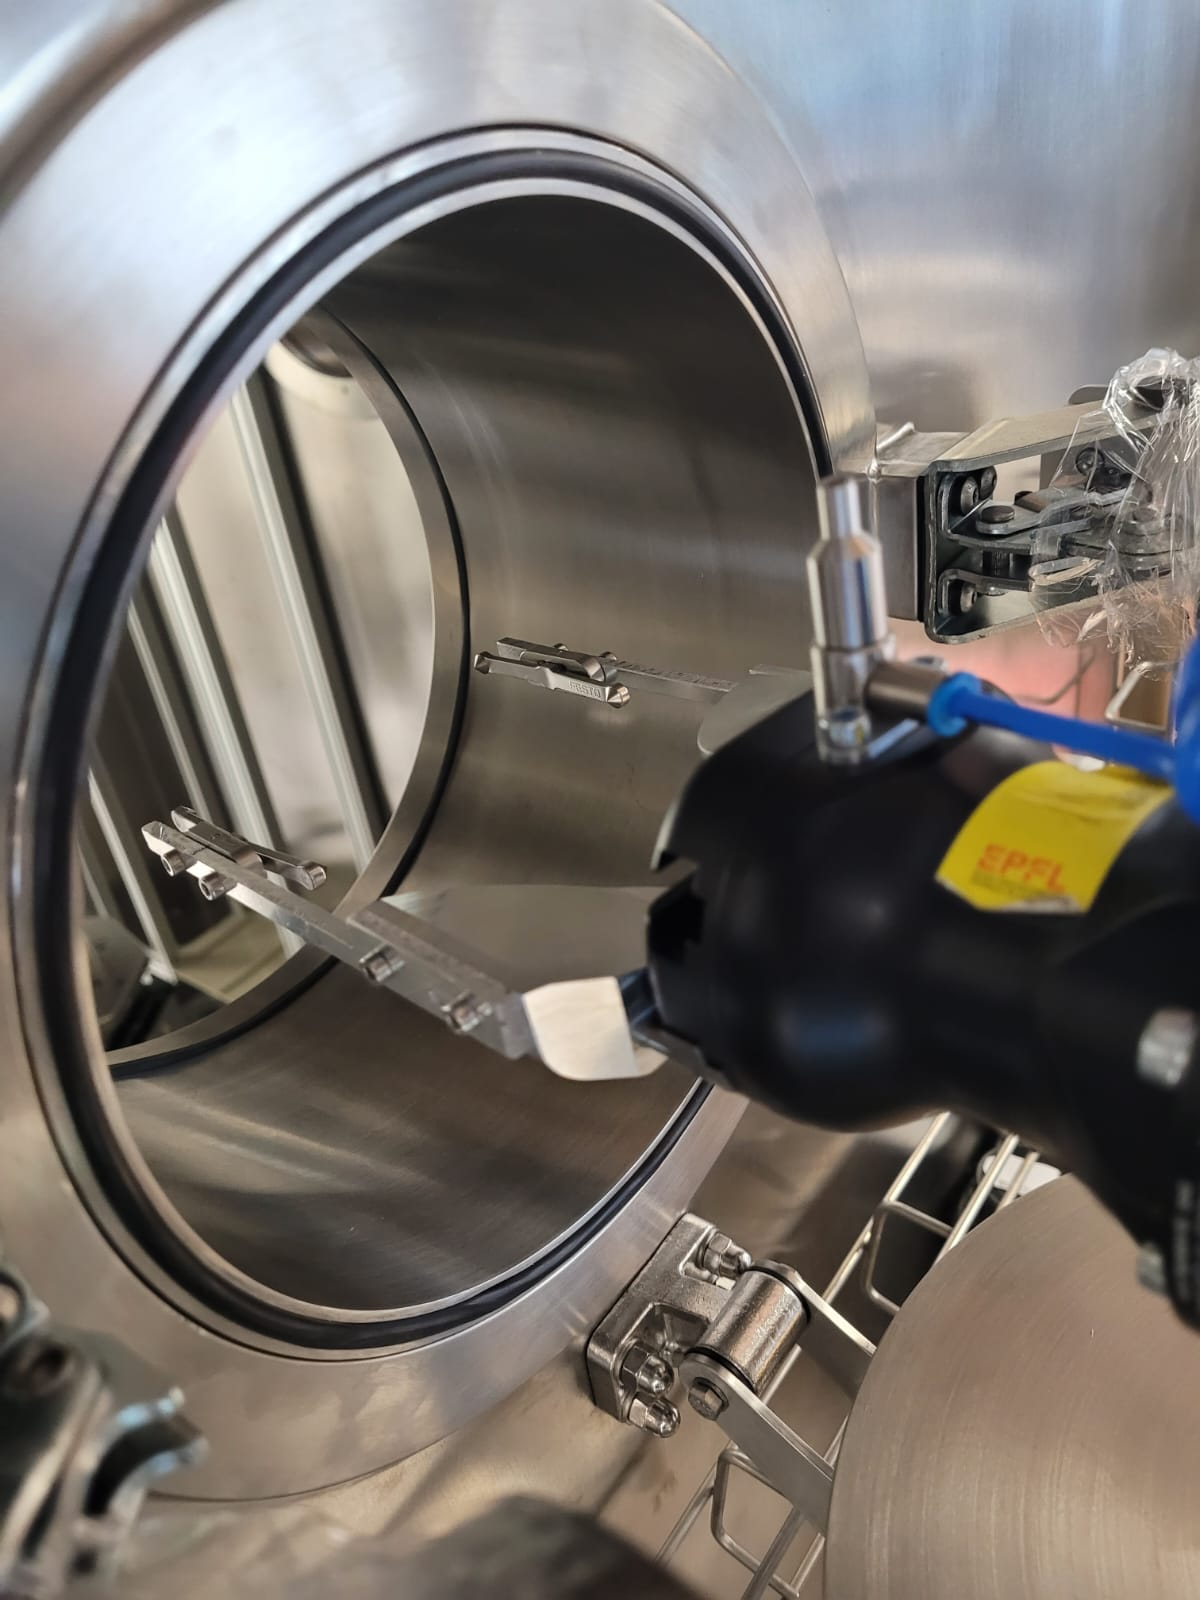
\includegraphics[width = 0.5\textwidth]{assets/figures/Hardware/outil_complet.jpeg}
    \caption{Module d'aspiration}
    \label{img:integration_pince}
\end{figure}